
\section{Multiparty garbled RAM: both database sizes}
\label{sec:garbled}
\textbf{Under the requested communication-bottleneck assumption, recurring
garbling preprocessing is the main traffic cost.} About 97.7\% of modeled bytes
are preprocessing, not the delivered garbled tables. SSD capacity can nevertheless
dominate the dollar bill if a long future execution is retained in full. The
reference policy below costs \$10.33--18.52B/year at $2^{28}$ records and
\$55.07--65.69B/year at $2^{32}$. Shortening the latter's prepared horizon reduces the
conditional estimate substantially. None of these ranges includes a measured,
finite OT-only correlation generator or a complete malicious epoch-renewal protocol.

\subsection{Scope and Boolean work ledger}
We use \emph{Multiparty Garbling from OT with Linear Scaling and RAM Support}
(ePrint 2025/444), including Appendix H and its tri-state encoding in Appendix F.
The local 49-page PDF was checked directly. The ten-party setting tolerates four
static malicious corruptions with abort. Field elements and labels have width
128 bits; this is a parameter choice, not a demonstrated 128-bit service-lifetime
failure bound.\footnote{\url{https://eprint.iacr.org/2025/444}. The retained local
source is \texttt{multiparty\_ot.pdf}; detailed equation notes are in
\texttt{data/garbling\_backend\_notes.txt}.}

As requested, all garbled-stack and associated adaptor costs are set to zero,
assuming the two-party improvement in ePrint 2026/761 can be migrated. That paper
optimizes the stack subroutine; it does not remove ordinary RAM reads, eviction,
recursive maps, or initialization. Its measured regime is two-party, up to
$2^{24}$ cells. Our extrapolation is consequently a conditional multiparty
construction, not a published benchmark.\footnote{\url{https://eprint.iacr.org/2026/761},
local \texttt{garbled\_merge.pdf}, final August revision, Sections 3.4, 5.3 and 6.2.
The public code artifact at \url{https://zenodo.org/records/20751401} supplies
the structural Circuit ORAM and recursive-map templates used here.}

\texttt{garbled\_circuit.py} counts Boolean AND and XOR work separately from the
interactive arithmetic model. The layout still has two $2N$-cell cuckoo arrays,
two fixed probes, exact 256-bit key comparisons, 256-bit output selection,
occupancy bits and an eight-entry dictionary stash. Each data payload has
513 bits. The main frontend accepts privately supplied hash indices, as in the
interactive comparison; exact key checks prevent a false hit. Two internal SHA3
hashes are priced separately. Malformed supplied indices can force a miss for
that client's query; internal hashing provides the stricter key-only functionality.
Position labels, conditional payload movement,
recursive block selection, and the final flat map are charged explicitly.

The source-inspired garbled tree has mostly four children per node; the
position-map packing fanout is a separate parameter. We sweep packing factors
2--128 and flat-base thresholds 16--4096, both powers of two, and the source's
compute- and communication-oriented stash/bucket/eviction choices. The selected
packing is eight for both sizes. These are source-derived circuit templates,
not counters from an executed ten-party implementation. Stash parameters and
lifetime failure probabilities still need validation at the larger sizes.

The distinction between \emph{visited} and \emph{generated} gates is essential.
For a horizon of $T$ logical KV queries, the source provisions $(1+E)T$ root
invocations, where $E$ is the number of extra evictions. Child budgets use rounded
division by the number of children, with a root-level $D/\mathrm{way}$ allowance
for a $D$-cell RAM, capped by the parent's budget. We sum every provisioned
node's circuit and divide by $T$. Summing only the online visited path underprices
the offline factory and SSD programme. Both probes are already in this count.

\subsection{What an AND gate costs with ten parties}
Let $A,I,O$ be generated AND gates, input bits and output bits, each amortized
per logical query in an epoch of $T$ queries. XOR is free in
communication, but still has local work. With outer packing $\ell=5$, the
ciphertext parameter is $c=\lceil10/5\rceil=2$. Each of the nine non-evaluators
sends
\[
 4(c+1)\cdot16=192\text{ bytes/AND};\qquad
 V_{\mathrm{table}}=9\cdot192A=1728A\text{ bytes}.
\]
The evaluator receives this aggregate. The additive mask in each row is a
\emph{field element}, not one bit. Appendix H's printed equation uses $n$ in
this final delivery term; the protocol sends from $i\ne1$, so we use $n-1$.
Charging every party 1728 bytes as its own transmitted table would overcount.
Appendix H prices Boolean circuits; Appendix F's full tri-state protocol has
additional preprocessing whose finite coefficient is not specified there.
We use H for Boolean RAM kernels and F for retained state, under the free
stack migration assumption. Any necessary non-stack, cross-gadget or
Boolean-to-tri-state conversion remains an unpriced compiler component;
ignoring the stack does not prove those conversions free.
This combined accounting template is not
an exact finite-cost instantiation of the paper's complete tri-state RAM protocol.

For finite preprocessing parameters, outer $\ell/n=0.5$ and the inner SuperPack
choice $k=3$, $\epsilon_{\mathrm{SP}}=0.4$ are distinct. They support the requested
threshold; substituting one common $\epsilon$ would obscure integer packing.
The leading global preprocessing traffic, with a conservative repair of the
paper's multiplication-count algebra, is
\[
 V_{\mathrm{prep}}=16(2747.5I+4618.5A+36O+1440/T)
 \quad\text{bytes/query.}
\]
Thus an AND contributes 73,896 global preprocessing bytes, or 7,389.6 bytes
averaged over the ten parties, before table delivery and framing. Input delivery
adds 434.25 bytes/bit globally and output delivery adds 288 bytes/bit. We use
$O=257$ (value and membership), and charge query/position inputs plus all initial
physical-state bits amortized over $T$. Shared randomness generation and valid
hidden state construction remain separate protocol obligations.

The repair is explicit: the first, exact line of Appendix H equation (8)
expands to three times its whole-circuit input count plus five times its AND
count, plus $1+\ell$ multiplication gates. Its approximation and later
equation (10) disagree; the latter uses $2I+4A$. Keeping that printed latter
choice instead gives $16(2575I+4446A+36O+1440/T)$ bytes/query. We show its effect below.
The once-per-circuit constant is amortized over an epoch; these are leading
counts, so remaining lower-order checks and protocol wrappers are not certified
finite costs.

\textbf{Correlation generation is an explicit unresolved cost.} The paper's
numerical ledger assumes efficient correlation generation; the OT-only variant
adds OLE correlations without a complete finite byte coefficient. Corrections
sent after receiving VOLE are not the cost of producing that VOLE. Our default
uses the reported leading ledger with negligible amortized correlation traffic.
The +25\% and +100\% preprocessing cases below are sensitivities, not measured
implementations or proven upper bounds. This prevents the estimate from being
misread as a fully priced OT-only malicious backend.

\subsection{Network capacity and SSD retention}
All parties together transmit $V$ bytes per query, including 5\% framing.
Let $s_i,r_i$ be party $i$'s sent/received bytes. Since AWS NIC bandwidth is
full duplex, its capacity demand is $\max(s_i,r_i)$, and
\[
 V\ \leq\ \sum_i\max(s_i,r_i)
   =V+\tfrac12\sum_i|s_i-r_i|\ \leq\ 2V.
\]
This gives a role-independent fleet envelope without assuming that preprocessing
traffic is perfectly balanced. It does not identify an actual assignment of
machines. We use \texttt{c6in.32xlarge}, 200 Gbps in each direction,
\$7.2576/hour, with efficiency factors $0.65\cdot0.70\cdot0.70$:
7.9625 GB/s per node per direction. At rate $R=10^4$, the fleet ranges from
$\max(10,\lceil RV/C\rceil)$ to
$\max(10,\lceil2RV/C\rceil+9)$ machines; the nine cover separate party ceilings.
Annual EC2 cost is machines times $8760\cdot\$7.2576$. The range describes
role imbalance only; it is not an uncertainty interval covering omitted costs.
The x86 SKU avoids assuming an ARM port.\footnote{Official AWS US East
(N. Virginia) feed snapshot \texttt{20261012193925}; raw selected rows and URLs
are in \texttt{data/aws\_garbled\_prices\_2026-10-13.json}.
\url{https://docs.aws.amazon.com/AWSEC2/latest/UserGuide/ec2-instance-network-bandwidth.html}.}

Same-AZ inter-party transfer has no marginal data-transfer fee under the chosen
placement. SSD capacity uses gp3 at \$0.08/GiB-month, or \$0.96/GiB-year. Per the
requested assumption we do not constrain SSD throughput or charge additional
provisioned IOPS/throughput. No inference about local evaluation speed is made.
CPU, EBS attachment/IO scheduling, AWS capacity and quotas need a deployment
validation before this resource envelope becomes a feasible service.
\footnote{\url{https://aws.amazon.com/ebs/pricing/}. AWS explicitly defines the
capacity-pricing GB unit as $2^{30}$ bytes. Network GB and plotted EB are decimal.}

Let $L$ be retained physical Boolean state bits, including bucket slack and
recursive maps. We retain the literal Appendix F packs: 224 bytes/bit at the
evaluator and 64 at each of the other nine parties, totaling $800L$ bytes.
This is a conservative policy; garbler packs can potentially be retired.
Only one aggregate copy of the garbled programme is charged, at the evaluator:
\[
 S_{\mathrm{one\ epoch}}=1728AT+800L,\qquad
 S_{\mathrm{reference}}=2S_{\mathrm{one\ epoch}}.
\]
The two copies represent the current and next prepared epoch for one independent
state. Preprocessing transcripts are not counted as retained programme. A
short streaming buffer would require a concrete scheduling argument, so it is
not silently substituted for a complete epoch.

\begin{center}\small\begin{tabular}{lrr}\toprule
Reference: $T=2N$, two complete epochs & Smaller database & Larger database\\\midrule
Logical records & $2^{28}$ & $2^{32}$ \\
Packing fanout / flat base & 8 / 256 & 8 / 512 \\
ANDs visited/query & 1.193M & 1.562M \\
ANDs generated/query & 1.288M & 1.672M \\
Prep. GB/query, all parties & 95.43 & 123.83 \\
Table GB/query, all parties & 2.23 & 2.89 \\
Framed sent GB/query, average party & 10.25 & 13.31 \\
Epoch length at 10k QPS & 14.91 h & 238.61 h \\
One epoch of tables, decimal EB & 1.195 & 24.815 \\
Two epochs + state, decimal EB & 2.394 & 49.711 \\
Network EC2/year & \$8.19--16.38B & \$10.62--21.25B \\
SSD capacity/year & \$2.14B & \$44.44B \\
Total/year, reference epoch & \$10.33--18.52B & \$55.07--65.69B \\
\bottomrule\end{tabular}\end{center}

\textbf{The throughput bottleneck here is offline communication, by assumption.}
Preprocessing is about 97.7\% of traffic; generated tables and encoded I/O account
for the rest. Even table delivery can occur before a query, so the remaining
2.3\% is not all online interaction. We have not measured whether computing the
preprocessing or evaluating the programme would overtake networking. A ready
garbling can have few online rounds while being very expensive to sustain at
10,000 queries/s. The large-size reference's SSD bill exceeds its network EC2
bill, making retention the largest dollar item despite the stipulated NIC
throughput bottleneck.

\subsection{Choose the prepared horizon rather than fixing it to database size}
An epoch of $T$ queries is an offline provisioning horizon, \emph{not} a batch
that must accumulate before answering. Smaller $T$ reduces retained tables but
amortizes fixed per-node invocation allowances and initial-state encoding over
fewer queries. We reoptimize the same finite layout grid at each power-of-two
horizon from $(2N)/256$ to $16(2N)$. The table shows representative points; all
points are saved in JSON.

\begin{center}\small\begin{tabular}{llrrrr}\toprule
Records & Queries/epoch & Hours & AND M/query & SSD \$B/year & Total/year\\\midrule
$2^{28}$ & $2^{23}$ & 0.23 & 2.740 & 0.08 & \$18.82--37.56B \\
$2^{28}$ & $2^{25}$ & 0.93 & 2.124 & 0.22 & \$14.04--27.85B \\
$2^{28}$ & $2^{27}$ & 3.73 & 1.581 & 0.66 & \$10.77--20.88B \\
$2^{28}$ & $2^{28}$ & 7.46 & 1.386 & 1.15 & \$9.99--18.83B \\
$2^{28}$ & $2^{29}$ & 14.91 & 1.288 & 2.14 & \$10.33--18.52B \\
$2^{28}$ & $2^{30}$ & 29.83 & 1.241 & 4.12 & \$12.00--19.88B \\
$2^{32}$ & $2^{27}$ & 3.73 & 3.346 & 1.46 & \$24.06--46.66B \\
$2^{32}$ & $2^{29}$ & 14.91 & 2.646 & 4.46 & \$21.59--38.71B \\
$2^{32}$ & $2^{31}$ & 59.65 & 2.012 & 13.42 & \$26.27--39.11B \\
$2^{32}$ & $2^{32}$ & 119.30 & 1.786 & 23.78 & \$35.15--46.52B \\
$2^{32}$ & $2^{33}$ & 238.61 & 1.672 & 44.44 & \$55.07--65.69B \\
$2^{32}$ & $2^{34}$ & 477.22 & 1.617 & 85.90 & \$96.17--106.43B \\
\bottomrule\end{tabular}\end{center}
Minimizing the \emph{upper endpoint} in this grid selects 14.91 hours at
$2^{28}$ and 14.91 hours at $2^{32}$, costing \$10.33--18.52B and \$21.59--38.71B/year,
respectively. These are conditional optima inside the chosen template and epoch
policy. The lower and upper fleet endpoints can prefer different horizons.
Do not treat the reference's large SSD footprint as an unavoidable lower bound
for garbled RAM.

\begin{center}
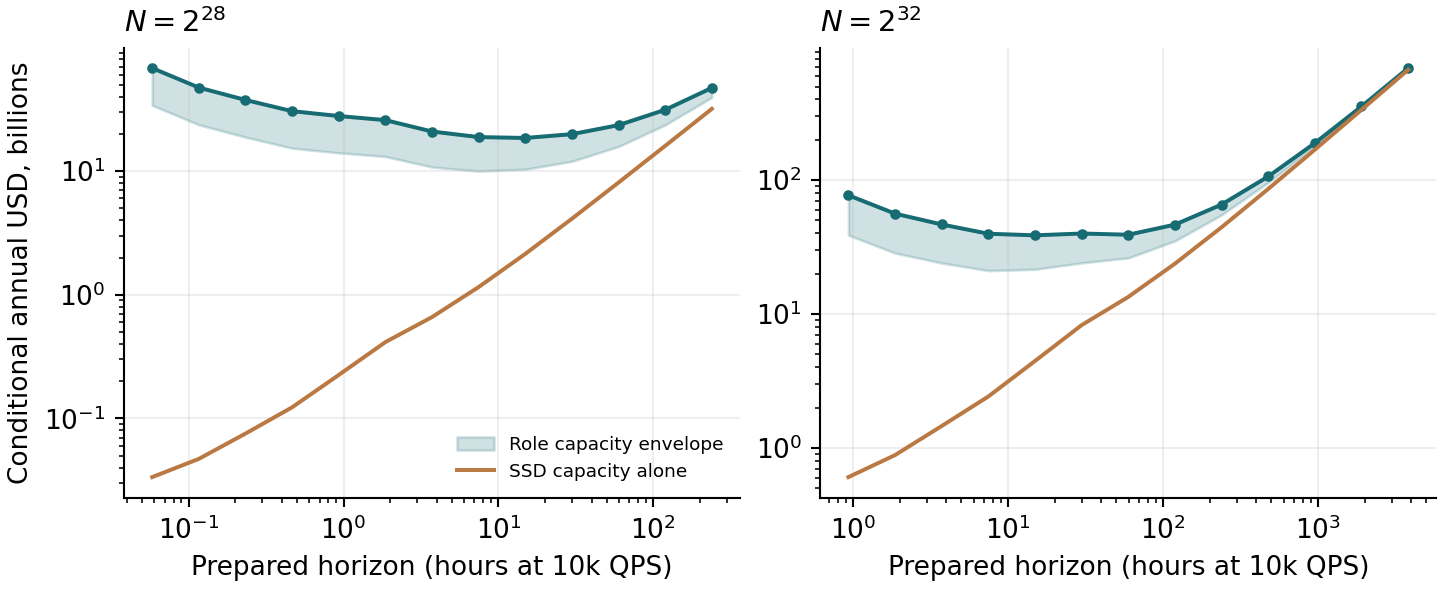
\includegraphics[width=\linewidth]{results/garbled_epoch_cost.png}
\end{center}
\textbf{Shorter epochs are not a solved free refresh.} Re-inputting existing
state pays for encoding; it does not compute a valid jointly hidden layout,
sample and validate private routing controls, or transfer a live state securely
to the next garbling. The two-party source knows controls at its sole garbler;
that role cannot simply be assigned to one possibly corrupted party here.
Also, the cited multiparty theorem uses static corruptions and standalone
function evaluation. Continuously injecting new, possibly adaptive external
client requests through an epoch needs a service-security argument. Internal
RAM adaptivity alone does not establish that API. These integration assumptions
apply at every horizon, including the reference.

\subsection{Sensitivity and comparison with interactive MPC}
\begin{center}\small\begin{tabularx}{\linewidth}{Xrr}\toprule
Change from the $T=2N$ reference & $N=2^{28}$ & $N=2^{32}$\\\midrule
Printed multiplication algebra & \$10.03--17.92B & \$54.68--64.92B \\
Additional correlation traffic: +25\% of prep. & \$12.33--22.52B & \$57.66--70.88B \\
Additional correlation traffic: +100\% of prep. & \$18.33--34.52B & \$65.45--86.46B \\
One complete epoch retained & \$9.26--17.45B & \$32.85--43.47B \\
Ten independent states, two epochs each & \$29.59--37.78B & \$455.07--465.70B \\
Compute two SHA3 hashes inside the circuit & \$10.94--19.62B & \$57.59--68.70B \\
Routing-only initialization allowance & \$12.78--22.91B & \$66.68--79.54B \\
All inter-party bytes cross AZs & \$657.09--665.28B & \$894.27--904.89B \\
\bottomrule\end{tabularx}\end{center}
Each row changes one assumption. The routing-only allowance applies a padded
Bene\v{s} permutation to every tree's physical slots with block width
$w+2h+1$: for $K$ padded slots, it charges $(K/2)(2\log_2 K-1)$ secret switches,
one AND per moved bit per switch, plus encoding the supplied control bits.
It excludes generation and verification of valid controls. Thus it is a concrete additional kernel, not a complete setup
budget. Ten states multiply SSD capacity while sharing the aggregate 10k QPS;
they do not multiply the same query traffic by ten. A one-epoch policy halves
retention, not recurring production cost. Cross-AZ traffic charges both billed
endpoints once per transmitted byte, at \$0.02/decimal GB in total.

The interactive reference costs \$2.33B/\$5.16B per year at the two sizes, with
modeled mean latencies 4.77/3.97 seconds. Its resource bottleneck is local
arithmetic, mostly online work under the baseline phase attribution; at $2^{32}$ RAM capacity also forces additional
machines. The garbled model instead gives a network/SSD resource envelope under
the user-specified network bottleneck, with costly recurring offline production.
We do not claim a five-second garbled-service latency without an evaluation and
scheduling benchmark. Both models include ten parties and sustainable repeated
query work, but their CPU assumptions and replica policies differ. These dollar
figures do not establish a universal protocol ranking.

For the proposal, retain interactive arithmetic compilation as the working
direction and state the concrete benchmark milestones. Neither this garbled
construction nor the unimplemented all-arithmetic reference currently supports
a low-cost production commitment. A tighter garbled estimate requires finite
malicious correlation costs, a joint initialization/renewal implementation,
reactive input handling, a concrete party traffic graph, and measured local
evaluation, including any representation adapters. SSD streaming and independent-state scheduling are additional
optimization opportunities rather than assumed free savings.
